\chapter{Related Work}
\label{chapter:related_work}

\section{Academic Work}

\subsection{Model-driven Development of Adaptive IoT Systems}

The paper with the title ``Model-driven Development of Adaptive IoT Systems''\cite{hussein2017model} shows how to develop adaptive \gls{ac:iot} systems using a model-driven approach.
Its approach is to first model state machines of all system components using SysML4IoT \cite{7592792}, then use a publish/subscribe architecture to model the environment information and the relationship within the system.
From these state machines then the source code is generated that can be deployed to the numerous \gls{ac:iot} devices.
Those devices then change their configuration at runtime (switching to another state), if the system sends them a message that contains information that leads to a state change based on the state machine implementation.
Also the system state is synchronized with the previously designed model.
This way the system state can be manually changed by changing the state of the model.

\subsubsection{Discussion}

The approach how to handle runtime configurations of this paper is very different to our approach.
This papers designs the system as a whole first, having the relations and adaptions of the nodes in this system in mind and also providing manual runtime configuration through its model.
This creates a system that can work very well on its own, but is not very good in ``integrating with the world''.
Our goal in this thesis is to create a \gls{ac:rcs} for an operating system (\gls{gl:riot_os}), that is constructed the other way around.
Not having the final system in mind, but providing standardized \glspl{ac:api} to allow writing mappings to many standardized external \glspl{gl:configuration_manager} or protocols like \gls{gl:lwm2m}.

\subsection{Architecting Emergent Configurations in the Internet of Things}

The paper with the title ``Architecting Emergent Configurations in the Internet of Things''\cite{7930220} explains the Emergent Configurations concept and proposes an architecture for its realization.
It further focuses on how Emergent Configurations are formed to achieve user's goals and how applications can adapt to runtime context changes.
The main idea behind Emergent Configurations is that all devices integrate with each other and change their configuration / behavior depending on other devices.
The paper gives a conference room as an example, which automatically adjusts its curtains if the projector is used and depending on what kind of media is presented and if it is properly visible or not.

\subsubsection{Discussion}

The connection between this work and the \gls{ac:rcs} for \gls{gl:riot_os} is, that it shows what can be achieved when having a well designed \gls{ac:rcs}, that uses shared \glspl{ac:cs} (see \autoref{sec:requirements:shared_pre_defined_configuraiton_schemas})).
Without these stable and reliable interfaces that a shared \gls{ac:cs} offers, it would be impossible for so many different devices to communicate so flawlessly as in this paper.

\subsection{CoAP Management Interface (CORECONF)}

The paper with the title ``CoAP Management Interface (CORECONF)'' \cite{draft-ietf-core-comi-11} specifies a ``network management interface for constrained devices and networks''.
It builds on \gls{ac:coap} to access resources specified in a \gls{ac:cbor} mapping of \acrshort{ac:yang} schemas \cite{RFC-6020} and also converts the \acrshort{ac:yang} identifier string to numeric identifiers to save payload size.
If specified, \acrshort{ac:yang} schemas can have multiple instances.

\subsubsection{Discussion}

This work is similar to the requirements specified in \autoref{chapter:requirements} of our thesis, in that it uses integers as a configuration resource identifier and uses shared configuration schemas (\acrshort{ac:yang}), which support multiple instances.
The paper differs to the requirements of our thesis in that it does not specify how these configuration changes should be applied / handled by the local (constrained) device itself.
The paper only specifies a protocol for how to do configurations through the network.
The introduced CORECONF protocol can be used for external configuration management of the new \gls{gl:riot_os} \gls{ac:rcs}.

\section{Implementation Work}

\subsection{Apache Mynewt: Config}
\label{sec:analysis:related_work:mynewt_config}

Mynewt is an embedded OS developed by the Apache Software Foundation.
It is similar to \gls{gl:riot_os} and already comes with a system module for runtime configurations, called ``Config'' \cite{apache-mynewt-20}.

It manages configuration parameters as key-value pairs of strings.
A key contains a path to a configuration parameter inside a module.
For example the key ``id/serial'' means the ``serial'' parameter of the ``id'' module.
So every module that uses \gls{ac:mynewt_config}, has its own namespace (initial module name, in this case ``id'') to put configuration data and how the configuration path is structured after the namespace is defined by each module itself.
For example the ``id'' module could have a configuration parameter under the ``id/serial/i2c/instance\_1'' path.
It is also possible to optionally persist configuration values to storage, so that configurations are not lost even after a restart of a device.

\subsubsection{Internal: Handler}

Each module needs to implement a so called ``handler'' so it can expose configuration parameters to \gls{ac:mynewt_config}.
These handlers have a simple \gls{ac:api}:

\paragraph*{``ch\_get'' Function}\mbox{}

This function takes a string key as its input and returns the configuration parameter's value as a string.

\paragraph*{``ch\_set'' Function}\mbox{}

This function takes a string key and a string value as its input and sets the configuration parameters value to the given value.

\paragraph*{``ch\_commit'' Function}\mbox{}

This function takes a string key as its input, which does not need to point to a concrete configuration parameter, but could also only point to the module itself or some shorter path, because this function will be executed on every configuration parameter, that is within this path.
For example the path ``id/serial'' includes ``id/serial/i2c'' and also ``id/serial/spi''.
This function takes changes that have been previously made by calling ``ch\_set'' into effect.
Just calling ``ch\_set'' only sets a value, but does not apply it.
This way multiple configuration parameter can be set to new values one by one and then are taken into effect at the same time.

\paragraph*{``ch\_export'' Function}\mbox{}

This function takes a string key and a callback function as its input, which does not need to point to a concrete configuration parameter, but could also only point to the module itself or some shorter path, because this function will be executed on every configuration parameter, that is within this path.
For example the path ``id/serial'' includes ``id/serial/i2c'' and also ``id/serial/spi''.
This function finds all configuration parameters, that are within the given path and exports them by calling the given callback function and passing their path and their value as an argument.

\subsubsection{API}
\label{sec:related_work:mynewt_api}

The \gls{ac:api} contains of 6 basic functions, that cover the most important use cases.
It also includes a few more functions for example to help converting configuration values to and from strings, but these are not important for our thesis.

\paragraph*{Get Configuration Values}\mbox{}

It is possible to get the value of a configuration parameter by calling the ``conf\_get\_value'' function.
Internally this function finds the ``handler'' by the first element of the given path and calls its ``ch\_get'' function.

\paragraph*{Set Configuration Values}\mbox{}

It is possible to set a value of a configuration parameter to a new value by calling the ``conf\_set\_value'' function.
Internally this function finds the ``handler'' by the first element of the given path and calls its ``ch\_set'' function.

\paragraph*{Transactionally Commit Configuration Values}\mbox{}

It is possible to commit configuration parameters by calling the ``conf\_commit'' function.
Internally this function finds the ``handler'' by the first element of the given path and calls its ``ch\_commit'' function.

\paragraph*{Save Configuration Values to Storage}\mbox{}

It is possible to save configuration parameters to storage by calling the ``conf\_save'' function.
Internally this function finds the ``handler'' by the first element of the given path and calls its ``ch\_export'' function, by giving a internal function as its callback value, that then gets called by the handler's export function and writes all the configuration parameters to storage.

\paragraph*{Load Configuration Values from Storage}\mbox{}

It is possible to load configuration parameters from storage by calling the ``conf\_load'' or ``conf\_load\_one'' function.
Internally these functions look into the storage and search for either, in case of ``conf\_load\_one'', for a specific configuration parameter, or in case of ``conf\_load'', for all available configuration parameters.
For each parameter, that is found in storage, the ``conf\_set\_value'' function is then called.

\subsection{Zephyr: Settings}

Zephyr is one of the most popular current IoT operating systems.
It is part of the Linux Foundation and backed by large companies such as Google, Meta, Intel and others \cite{zephyr-20}.
Given its huge success, it is interesting to see how this rather large competitor handles runtime configuration.
The system module responsible for runtime configuration within the Zephyr operating system is called Zephyr Settings \cite{zephyr_settings_pull_request} and an implementation of \gls{ac:mynewt_config} \cite{apache-mynewt-20}.
Both \glspl{ac:api} are mostly the same but have some minor differences.

Zephyr Settings vs. \gls{ac:mynewt_config} - \gls{ac:api} Comparison:

\paragraph*{Get Configuration Values}\mbox{}

\autoref{table:mynewt_vs_zephyr_read} shows the similarities between the ``get'' functions of \gls{ac:mynewt_config} and Zephyr Settings.
The only real differences besides the usage of different names being that Zephyr settings returns an integer, while \gls{ac:mynewt_config} returns a char pointer and that the Zephyr settings \gls{ac:api} does not limit itself to passing only strings, but accepts a void pointer and has an additional ``len'' parameter, containing the size of the value.

\begin{table}[H]
      \begin{tabular}{ | l | l | }
            \hline
            M. Config   & char *conf\_get\_value(char *name, char *buf, int buf\_len);
            \\ \hline
            Z. Settings & int settings\_runtime\_get(const char *name, void *data, size\_t len);
            \\
            \hline
      \end{tabular}
      \caption{M. Config vs. Z. Settings: Read}
      \label{table:mynewt_vs_zephyr_read}
\end{table}

\paragraph*{Set Configuration Values}\mbox{}

\autoref{table:mynewt_vs_zephyr_write} shows the similarities between the ``set'' functions of \gls{ac:mynewt_config} and Zephyr Settings.
The only real differences besides the usage of different names being that Zephyr settings \gls{ac:api} does not limit itself to passing only strings, but accepts a void pointer and has an additional ``len'' parameter, containing the size of the new value.

\begin{table}[H]
      \begin{tabular}{ | l | l | }
            \hline
            M. Config   & int conf\_set\_value(char *name, char *val\_str);
            \\ \hline
            Z. Settings & \begin{tabular}[l]{@{}l@{}}int settings\_runtime\_set(const char *name, const void *data,\\size\_t *len);\end{tabular}
            \\
            \hline
      \end{tabular}
      \caption{M. Config vs. Z. Settings: Write}
      \label{table:mynewt_vs_zephyr_write}
\end{table}

\paragraph*{Transactionally Commit Configuration Values}\mbox{}

\autoref{table:mynewt_vs_zephyr_apply} shows the similarities between the ``commit'' functions of \gls{ac:mynewt_config} and Zephyr Settings.
The only real differences besides the usage of different names being that Zephyr settings \gls{ac:api} uses a const parameter.

\begin{table}[H]
      \begin{tabular}{ | l | l | }
            \hline
            M. Config   & int conf\_commit(char *name);
            \\ \hline
            Z. Settings & int settings\_runtime\_commit(const char *name);
            \\
            \hline
      \end{tabular}
      \caption{M. Config vs. Z. Settings: Apply}
      \label{table:mynewt_vs_zephyr_apply}
\end{table}

\paragraph*{Load Configuration Values from Storage}\mbox{}

\autoref{table:mynewt_vs_zephyr_load} shows the similarities between the ``load'' functions of \gls{ac:mynewt_config} and Zephyr Settings.
The only real differences is the usage of different names.

\begin{table}[H]
      \begin{tabular}{ | l | l | }
            \hline
            M. Config   & int conf\_load(void);
            \\ \hline
            Z. Settings & int settings\_load(void);
            \\
            \hline
      \end{tabular}
      \caption{M. Config vs. Z. Settings: Load}
      \label{table:mynewt_vs_zephyr_load}
\end{table}

\autoref{table:mynewt_vs_zephyr_load_a_single_parameter} shows the similarities between the ``load\_one'' functions of \gls{ac:mynewt_config} and Zephyr Settings.
The only real differences besides the usage of different names being that Zephyr settings \gls{ac:api} uses a const parameter.

\begin{table}[H]
      \begin{tabular}{ | l | l | }
            \hline
            M. Config   & int conf\_load\_one(char *name);
            \\ \hline
            Z. Settings & int settings\_load\_subtree(const char *subtree);
            \\
            \hline
      \end{tabular}
      \caption{M. Config vs. Z. Settings: Load a single parameter}
      \label{table:mynewt_vs_zephyr_load_a_single_parameter}
\end{table}

\paragraph*{Save Configuration Values to Storage}\mbox{}

\autoref{table:mynewt_vs_zephyr_save} shows the similarities between the ``save'' functions of \gls{ac:mynewt_config} and Zephyr Settings.
The only real differences is the usage of different names.

\begin{table}[H]
      \begin{tabular}{ | l | l | }
            \hline
            M. Config   & int int conf\_save(void);
            \\ \hline
            Z. Settings & int settings\_save(void);
            \\
            \hline
      \end{tabular}
      \caption{M. Config vs. Z. Settings: Save}
      \label{table:mynewt_vs_zephyr_save}
\end{table}

\autoref{table:mynewt_vs_zephyr_save_a_single_parameter} shows the similarities between the ``save\_one'' functions of \gls{ac:mynewt_config} and Zephyr Settings.
The only real differences besides the usage of different names being that Zephyr settings \gls{ac:api} does not limit itself to passing only strings, but accepts a void pointer and has an additional ``len'' parameter, containing the size of the new value.

\begin{table}[H]
      \begin{tabular}{ | l | l | }
            \hline
            M. Config   & int conf\_save\_one(const char *name, char *var);
            \\ \hline
            Z. Settings & \begin{tabular}[l]{@{}l@{}}int settings\_save\_one(const char *name, const void *value,\\size\_t val\_len);\end{tabular}
            \\
            \hline
      \end{tabular}
      \caption{M. Config vs. Z. Settings: Save a single parameter}
      \label{table:mynewt_vs_zephyr_save_a_single_parameter}
\end{table}

\subsection{\gls*{gl:lwm2m} Object and Resource Registry}
\label{sec:analysis:related_work:lwm2m}

While \gls{gl:lwm2m} by itself is a protocol for external runtime configuration management and not an operating system registry, it still has some appealing aspects that are relevant to the \nameref{sec:design:riot_registry}.
Besides the fact that the \nameref{sec:design:riot_registry} is supposed to integrate external \glspl{gl:configuration_manager} such as \gls{gl:lwm2m}.
Furthermore, it is to be evaluated if an \gls{gl:lwm2m} client such as Eclipse Wakaama \cite{eclipse_wakaama} can be used as the official \gls{gl:riot_os} configuration registry.
This way \gls{gl:lwm2m} is supposed to become the standard for \gls{gl:riot_os} configuration management and other management systems count integrate with \gls{gl:lwm2m} instead of a \gls{gl:riot_os}-specific registry.

\subsubsection{Predefined and typed object definitions}

\gls{gl:lwm2m} comes with its own predefined object definitions.
Each object definition has its own unique ID, name, and other metadata and contains multiple properties (configuration parameters) that describe the object and can be read (or written) to.
The properties themselves can not contain further child properties.
So the property list of an object definition is always flat.
Each property has an ID, a name, a type such as Integer, Boolean, String etc. and other metadata.
For example, there is the object with the ID 3420.
Its name is ``LED color light'' and it has one property ``RGB value'' with the ID 1.
This property has the type String and expects a color in the RGB hex format (\#rrggbb).

\subsubsection{Multiple instances}

The \gls{gl:lwm2m} protocol allows an object definition to have multiple instances.
So multiple modules/drivers can implement the same \gls{gl:lwm2m} object or expose multiple instances of themselves that will be accessible at the same time.
For example, a smart lamp might have multiple LEDs that all expose the same interface, but should be addressed individually to enable the mixing of different colors.

\subsubsection{Integer Resource Path}

To identify a property of some object \gls{gl:lwm2m} uses a path of 3 integers.
First comes the object ID, which is the ID of the object definition.
Second comes the instance ID which is the ID of the very instance of that object, since there can be multiple instances of each object.
And last comes the property ID.

\subsection{Prior Work on \gls*{gl:riot_os}}

Before the work on this thesis started, there has already been an initial implementation of \gls{ac:mynewt_config} (see \autoref{sec:analysis:related_work:mynewt_config}) for \gls{gl:riot_os} as an open PR on its GitHub repository (see PR 10622 \cite{riot_pr_10622} and PR 10799 \cite{riot_pr_10799}).

\section{Assessment of Implementation Work on Thesis's \acrshort{ac:rcs} Requirements}
\label{sec:related_work:assessment_of_implementation_work_on_thesis_requirements}

Besides \gls{gl:riot_os} there are other operating Systems such as Zephyr \cite{zephyr-20}, that may already provide solutions for managing runtime configurations in IoT.
So to find a suitable architecture to manage runtime configurations in \gls{gl:riot_os}, it is important to evaluate, if related work already exists, that can fully satisfy all the needs listed in \autoref{chapter:requirements}.
Besides that, it is important to learn the benefits and drawbacks of related tools to then decide whether to implement an already existing architecture into \gls{gl:riot_os} or to invent a new architecture that can benefit from what was learned while evaluating the work done in competing architectures.

\subsection{Apache Mynewt Config Subsystem}
\label{sec:related_work:mynewt_config}

\subsubsection{Advantages}
\label{sec:related_work:mynewt_config_advantages}

\begin{itemize}
      \item \textbf{\acrlongpl{ac:cs} can have a deeply nested tree structure}\\
            (see \autoref{sec:requirements:nested_configuration_groups})\\
            The configuration parameter identifier of each handler is stored as a simple string key.
            This makes it possible to easily have implicit grouping by just defining a long string with multiple separators.
            Then internally common groups of multiple parameters can be processed by the configuration subsystem.

      \item \textbf{Low implementation effort for modules/drivers}\\
            (see \autoref{sec:requirements:low_implementation_effort_for_modules_and_drivers})\\
            Every module just implements a set and get function inside a handler, that has gets or returns values as strings based on the input string, which is the identifier of a configuration parameter or group.

      \item \textbf{Easy integration with some other external \glspl{gl:configuration_manager}}\\
            (see \autoref{sec:requirements:integration_with_external_configuration_managers})\\
            Some tools that can be used for external \glspl{gl:configuration_manager} such as \gls{ac:coap} and \gls{gl:mqtt} for example can just reuse the configuration parameter path strings as address or topic.
            They can be written once and don't need to be implemented for every module (handler) of the configuration subsystem.

      \item \textbf{Transactionally Commit Configuration Changes}\\
            (see \autoref{sec:requirements:binary_internal_configuration_parameter_format})\\
            \gls{ac:mynewt_config} can transactionally commit multiple configuration changes at once my calling the ``commit'' function (see \autoref{sec:related_work:mynewt_api}).

      \item \textbf{Persistent Configurations}\\
            (see \autoref{sec:requirements:binary_internal_configuration_parameter_format})\\
            \gls{ac:mynewt_config} can persistently save configuration values to a non-volatile storage device by calling the ``conf\_save'' function (see \autoref{sec:related_work:mynewt_api}).
\end{itemize}

\subsubsection{Disadvantages}

\begin{itemize}
      \item \textbf{\acrlongpl{ac:cs} are defined per module/driver}\\
            (see \autoref{sec:requirements:shared_pre_defined_configuraiton_schemas})\\
            There are no shared configuration structure definitions that can be implemented by different modules.
            Each module implements its own custom configuration structure.
            Even if there are 2 different LED drivers, that do exactly the same except they use different hardware, they have no shared code.

      \item \textbf{No support for multiple instances}\\
            (see \autoref{sec:requirements:multiple_instances_per_schema})\\
            The subsystem itself has no construct for how instances might work.
            The implementing module/driver can of course hack around this by implementing an instance group as part of the path inside the handler and then internally map it to the duplicated devices that shall be configured.
            But this is a custom solution that will only make the configuration subsystem unnecessarily complex and inconsistent.

      \item \textbf{Path to configuration parameters as string}\\
            (see \autoref{sec:requirements:integer_path_as_identifier_of_configuration_values})\\
            The identifier of a configuration parameter is a string, which supports nested groups via ``/'' separators.
            In general, the structure of this string can be totally custom per module/driver, as the modules that implement a configuration handler decide how to interpret its structure.
            This causes a lot of overhead in string deserialization and is easy to cause errors or undocumented inconsistencies.

      \item \textbf{Configuration parameters have no type information}\\
            (see \autoref{sec:requirements:typed_configuration_parameters})\\
            Everything is based on strings.
            The handler implemented by the module must convert the input string into whatever format it needs.
            And also the other way around on return.
            In that sense, a type is not needed, as the handler takes care of it with the cost of performance overhead and a more complicated \gls{ac:api} for the user.
            If there are types the user could for example know if a number is needed or a string, which can be unclear in some scenarios.
            But this is not the case with this configuration subsystem.

      \item \textbf{Configuration parameter values are stored in the string format}\\
            (see \autoref{sec:requirements:binary_internal_configuration_parameter_format})\\
            As every parameter value is returned and set as a string value, it also is necessary to persist it as a string, so that the handler could understand it when it gets read and passed to it.
            As strings in most cases use up more storage than primitive values such as numbers, this can be a problem for constrained devices with not a lot of memory.

      \item \textbf{Difficult or almost impossible integration with some other external \glspl{gl:configuration_manager}}\\
            (see \autoref{sec:requirements:integration_with_external_configuration_managers})\\
            External \glspl{gl:configuration_manager} such as \gls{gl:lwm2m} have their predefined \gls{ac:cs} structure called object models.
            There is for example an object model for a colored light bulb.
            If this external \gls{gl:configuration_manager} is integrated with the \gls{ac:mynewt_config}, it is necessary to write a mapping for each \gls{ac:mynewt_config} handler to the corresponding object model in \gls{gl:lwm2m}.
            Considering that \gls{gl:lwm2m} is not the only standard for configuration management this becomes an issue to maintain.
            Also, some other simpler \glspl{gl:configuration_manager} could depend on integer arrays as an identifier for the configuration parameter.
            Transforming a string as is used in the parameter of the \gls{ac:mynewt_config}, will always have collisions and is therefore not reliable.
\end{itemize}

\subsubsection{Conclusion}

What is needed is not a registry that is split into modules/drivers, but a registry that defines data structures that can be implemented by multiple modules/drivers to share the same interface for identical use cases.

\subsection{\gls*{gl:lwm2m} Object and Resource Registry}
\label{sec:related_work:lwm2m}

\subsubsection{Advantages}

\begin{itemize}
      \item \textbf{\acrlongpl{ac:cs} are shared between modules/drivers}\\
            (see \autoref{sec:requirements:shared_pre_defined_configuraiton_schemas})\\
            \gls{gl:lwm2m} has predefined \glspl{ac:cs} for common use cases such as \acrshort{ac:wlan} configuration \cite{oma-lwm2m-core-12} or location data \cite[p. 124]{oma-lwm2m-core-12} called object models.
            Modules/drivers can implement these object models and in this way share the same data structure across similar use-cases.

      \item \textbf{Multiple \acrlongpl{ac:si}}\\
            (see \autoref{sec:requirements:multiple_instances_per_schema})\\
            Each \gls{gl:lwm2m} object model can be implemented and instantiated by more than one model/driver.
            To identify different instances, the instance\_id is part of the integer path to access configuration parameters: Object model/instance/parameter.

      \item \textbf{Path to configuration parameter as array of 3 integers}\\
            (see \autoref{sec:requirements:integer_path_as_identifier_of_configuration_values})\\
            The path to identify a single configuration parameter consists of 3 integers:
            Object Model ID / Instance ID / Parameter ID. This way the payload for requests will not be increased only because an object model has a long name.

      \item \textbf{Configuration parameters have type information}\\
            (see \autoref{sec:requirements:typed_configuration_parameters})\\
            A configuration parameter can have multiple types:
            String, (Unsigned) Integer, Float, Boolean, Opaque, Time \cite[p. 99]{oma-lwm2m-core-12}.
            This helps the user to find out what kind of value is valid for a given configuration parameter.

      \item \textbf{Configuration parameter values can have any internal type (string, int, binary, etc.)}\\
            (see \autoref{sec:requirements:binary_internal_configuration_parameter_format})\\
            The values of configuration parameters get set in their primary type and not formatted in some higher type such as a ``string type'' for example.

      \item \textbf{Transactionally Commit Configuration Changes}\\
            (see \autoref{sec:requirements:binary_internal_configuration_parameter_format})\\
            \gls{gl:lwm2m} has the ability to set multiple configuration parameters at once.
            If they are set at once, they would also be committed at the same time.

      \item \textbf{Persistent Configurations}\\
            (see \autoref{sec:requirements:binary_internal_configuration_parameter_format})\\
            The open source \gls{gl:lwm2m} client implementation called Eclipse Wakaama \cite{eclipse_wakaama} does not come with this feature, but it is possible to implement this functionality on top of it.
\end{itemize}

\subsubsection{Disadvantages}

\begin{itemize}
      \item \textbf{\acrlongpl{ac:cs} can not have a deeply nested tree structure}\\
            (see \autoref{sec:requirements:nested_configuration_groups})\\
            More complicated object models with many configuration parameters that can be logically structured, will have some unnecessary overhead.
            A structure can still be simulated by giving names such as:
            ``group\_a/group\_b/param\_c'' as parameter names.

      \item \textbf{High implementation effort for modules/drivers}\\
            (see \autoref{sec:requirements:low_implementation_effort_for_modules_and_drivers})\\
            The open source \gls{gl:lwm2m} client implementation called Eclipse Wakaama \cite{eclipse_wakaama} has a high implementation effort for module/driver developers to integrate it.
            For instance, the example implementation in the Wakaama Repository of the \gls{gl:lwm2m} location object model \cite[p. 125]{oma-lwm2m-core-12}, which only exposes 7 values(latitude, longitude, altitude, radius, velocity, timestamp and speed), already needs 352 lines of code \cite[p. 125]{oma-lwm2m-core-12}.

      \item \textbf{Difficult to integrate with other external \glspl{gl:configuration_manager}}\\
            (see \autoref{sec:requirements:integration_with_external_configuration_managers})\\
            \gls{gl:lwm2m} is itself an external \gls{gl:configuration_manager} and not intended as a middleware that could be integrated with other external \gls{gl:configuration_manager} tools.
            As a consequence, even though possible, the integration of other configuration tools with for example the ``Eclipse Wakaama'' client \cite{eclipse_wakaama}, which already requires considerably a lot of work to integrate itself as explained earlier, is not easily done.
            Most importantly to create good external \gls{gl:configuration_manager} integrations it is important to use meta-fields such as ``name'', or ``description''.
            Those fields exist in the \gls{gl:lwm2m} Object Model Definitions \cite[p. 68]{oma-lwm2m-core-12}, but these are only known by the \gls{gl:lwm2m} Server and not part of the \gls{gl:lwm2m} client running on the \gls{gl:riot_os} node \cite{oma-lwm2m-core-12}.
            This way the client cannot expose any human-readable information of its \gls{ac:api}, except integer paths and types.
\end{itemize}

\subsubsection{Conclusion}

Other \glspl{gl:configuration_manager} should be supported also. \gls{gl:lwm2m} is difficult to integrate with other managers.
An interface between \gls{gl:riot_os} and \gls{gl:lwm2m} is needed. For example, a new system module called \nameref{sec:design:riot_registry}.

\section{Summary of Implementation Work Assessment}
\label{sec:related_work:summary}

As \autoref{fig:related_work_influences} shows, there is a lot to be learned from existing technologies.
Especially in how different their approaches to fixing similar issues are.
But not only \gls{ac:mynewt_config} but also OMA \gls{gl:lwm2m} both on their own do not satisfy the needs of a \gls{gl:riot_os}-wide registry good enough, to be implemented as a solution to the problem.

The main issue with \gls{ac:mynewt_config} is the fact that each module would need to implement the \gls{ac:cs} on its own, which results in many similar but not identical \glspl{ac:cs} inside similar modules/drivers and also prevents the integration of external \glspl{gl:configuration_manager} such as \gls{gl:lwm2m} (see \autoref{sec:related_work:mynewt_config_advantages}).
Also, the lack of type information for configuration parameters makes the integration of external \glspl{gl:configuration_manager} that rely on type information problematic.

On the other hand, the main issues with OMA \gls{gl:lwm2m} are a way too large module implementation boilerplate and the high difficulty to integrate other external configuration managers with the local \gls{gl:lwm2m} schema.

\begin{figure}[H]
      \centering
      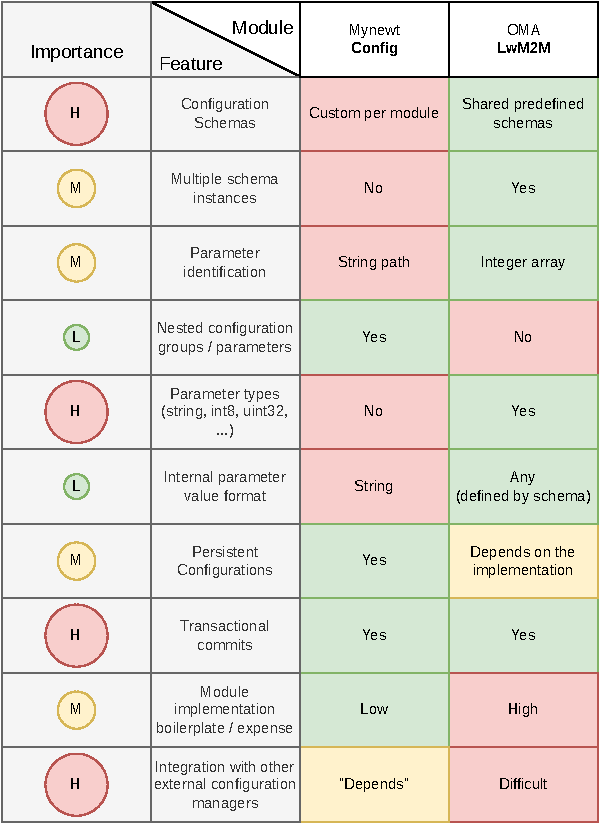
\includegraphics[width=\textwidth]{related_work_influences}
      \caption{Related work influences.}
      \label{fig:related_work_influences}
\end{figure}

\section{Conclusion of Implementation Work Assessment}
\label{sec:related_work:conclusion}

The logical consequence is the creation of a new configuration registry that is based on the concepts of \gls{ac:mynewt_config} and \gls{gl:lwm2m} but only uses those that fit the needs of the \gls{gl:riot_os} most.
It is supposed to keep the simplicity of the \gls{ac:mynewt_config}, by also supporting the advantages of OMA \gls{gl:lwm2m}.
The OMA \gls{gl:lwm2m} configuration manager can then be implemented through a mapping between the new \nameref{sec:design:riot_registry} configuration parameters and the \gls{gl:lwm2m} object models.

As can be seen on the right-hand side of \autoref{fig:related_work_conclusion}.
This new \nameref{sec:design:riot_registry} allows the specification of \glspl{ac:cs} that are shared by drivers and modules so that every driver or module that represents the same functionality will also have the same structural representation of their configuration parameters.
This also easily allows the ability to create multiple instances of the same \gls{ac:cs}.
For example, a traffic light would need 3 LEDs that use the same \gls{ac:cs}.
The identification of a configuration parameter of the \nameref{sec:design:riot_registry} is a result of its path, which is an array of integers, of which the length depends on how deeply nested the \gls{ac:cs} structure is.
To improve the integration of typed configuration managers, the configuration parameters also have metadata containing type information, but also strings such as ``name'' or ``description'' to allow the creation of more simple \glspl{ac:api} for developers.
For example a \gls{ac:cli} that allows using the name field as an alias to the integer array.
Internally the \nameref{sec:design:riot_registry} allows the \gls{ac:cs} to use every available type in the C programming language to specify the value of a configuration manager that is written to the program storage.
To prevent unnecessary conversion from string to native value and the other way around. The integration of the new registry into drivers or modules is also supposed to be as simple as possible.
Therefore, an \gls{ac:api} that is inspired by the \gls{ac:mynewt_config} (see \autoref{sec:analysis:related_work:mynewt_config}) will be implemented.

\begin{figure}[H]
      \centering
      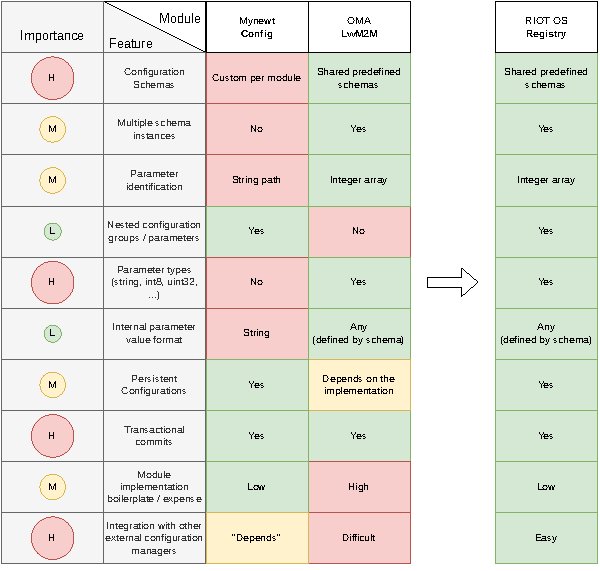
\includegraphics[width=\textwidth]{related_work_conclusion}
      \caption{Related work conclusion.}
      \label{fig:related_work_conclusion}
\end{figure}
